
\RequirePackage{fix-cm}
\documentclass[smallextended]{svjour3}       % onecolumn (second format)
\smartqed  % flush right qed marks, e.g. at end of proof

\usepackage{bussproofs}
\usepackage{turnstile}
\usepackage{amssymb}
\usepackage{latexsym}
\setcounter{tocdepth}{3}
\usepackage{graphicx}
\usepackage{url}
\usepackage{amsmath}
\usepackage{listings}
\usepackage{subfig}
\usepackage{pgf}
\usepackage{tikz}
\usetikzlibrary{arrows,shapes,snakes,automata,backgrounds,petri}
\usepackage[latin1]{inputenc}
\usepackage{float}
\usepackage{amssymb}

\lstnewenvironment{code}
    {\lstset{}%
      \csname lst@SetFirstLabel\endcsname}
    {\csname lst@SaveFirstLabel\endcsname}
    \lstset{
      basicstyle=\small\ttfamily,
      flexiblecolumns=false,
      basewidth={0.5em,0.45em},
      literate={+}{{$+$}}1 {/}{{$/$}}1 {*}{{$*$}}1 {=}{{$=$}}1
               {>}{{$>$}}1 {<}{{$<$}}1 {\\}{{$\lambda$}}1
               {\\\\}{{\char`\\\char`\\}}1
               {->}{{$\rightarrow$}}2 {>=}{{$\geq$}}2 {<-}{{$\leftarrow$}}2
               {<=}{{$\leq$}}2 {=>}{{$\Rightarrow$}}2 
               {\ .}{{$\bigcirc$}}2 {\ .\ }{{$\bigcirc$}}2
               {>>}{{>>}}2 {>>=}{{>>=}}2
               {|}{{$\mid$}}1               
    }

\newtheorem{mycase}{Case}
\newtheorem{subcase}{Case}
\numberwithin{subcase}{mycase}


% Dot
\def\fDot {\ast}
% Bang
\def\fBang {\ ! \ }
% Or
\def\fOr {\ | \ }

% Turnstiles with subscripts
\def\judgeX {\sststile{\mathrm{X}}{}}
\def\judgeY {\sststile{\mathrm{Y}}{}}
\def\judge {\sststile{\mathrm{}}{}}

\EnableBpAbbreviations



\begin{document}

\title {Eremic Logic} 
\subtitle {A Modal Logic of Elementary Propositions}
\author{Richard Prideaux Evans,  Martin Berger}
\date{Received: date / Accepted: date}
% The correct dates will be entered by the editor

\maketitle

\section{EL$[\land, !]$}
\subsection{Syntax}
Given a set $\mathcal{S}$ of symbols, with $a$ ranging over $\mathcal{S}$, and $A$ ranging over finite subsets of $\mathcal{S}$, the sentences of EL$[\land, !]$ are given by:
\[
\phi ::= \top \fOr \phi_1 \land \phi_2  \fOr \langle a \rangle \phi \fOr \fBang A 
\]
The $!$ operator is used to restrict the allowable transitions coming out of a state.
Intuitively, $\fBang A$ means that the \emph{only} transitions coming out of the current state are those specified in $A$.
\subsection{Semantics}
\begin{definition}
A {\bf model} is a triple $(\mathcal{W}, \rightarrow, \lambda)$, containing a Labeled Transition System (a set of states $\mathcal{W}$, and a transition relation $\rightarrow \; \subseteq \; \mathcal{W} \times \mathcal{S} \times \mathcal{W}$), together with a node-labelling $\lambda$ that maps each element of $\mathcal{W}$ to a subset of $\mathcal{S}$. 
\end{definition}
The intended interpretation is that $\lambda(w)$ is the set of allowed transition symbols emanating from $w$.
The $\lambda$ function is the semantic counterpart of the $!$ operator.

Now, for a model to be valid, we insist that the transitions coming out of a node $w$ are a subset of the allowed transitions in $\lambda(w)$:
\begin{definition}
A model $(\mathcal{W}, \rightarrow, \lambda)$ is {\bf valid} iff for all $w \in \mathcal{W}$, $ \{s \fOr \exists w' \; w \xrightarrow{s} w'\} \subseteq \lambda(w)$.
\end{definition}

\begin{definition}
A {\bf pointed model} is a pair $(l,w)$, where $m$ is a \emph{valid} model of the form $(\mathcal{W}, \rightarrow, \lambda)$, and $w$ is a distinguished state in $\mathcal{W}$.
\end{definition}
Formulae are interpreted in a pointed model $(l,w)$:
\begin{eqnarray}
(l,w) & \models & \top  \mbox{ always } \nonumber \\
(l,w) & \models & \phi_1 \land \phi_2 \mbox{ iff } (l,w)  \models \phi_1 \mbox { and } (l,w) \models \phi_2 \nonumber \\
(l,w) & \models & \langle a \rangle \phi \mbox{ iff there is a } w \xrightarrow{a} w' \mbox { such that } (l,w') \models \phi \nonumber \\
(l,w) & \models & \fBang A \mbox{ iff } \lambda(w) \subseteq A\nonumber
\end{eqnarray}
Note that if a model is valid then $(l,w) \models \fBang A$ implies $\{s \fOr \exists w' \; w \xrightarrow{s} w'\} \subseteq A$.
From now on, we will restrict ourselves to valid models.
\begin{figure}[h]
\centering
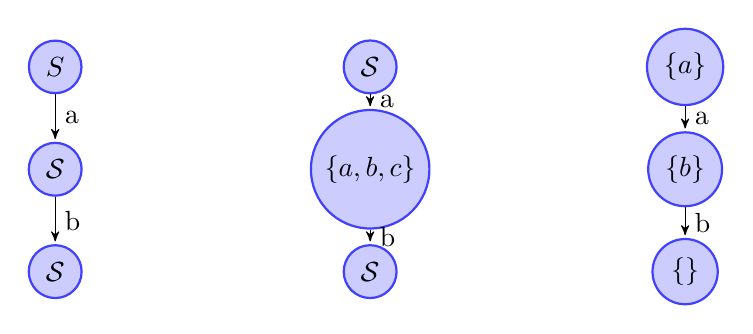
\begin{tikzpicture}[node distance=1.3cm,>=stealth',bend angle=45,auto]
  \tikzstyle{place}=[circle,thick,draw=blue!75,fill=blue!20,minimum size=6mm]
  \tikzstyle{red place}=[place,draw=red!75,fill=red!20]
  \tikzstyle{transition}=[rectangle,thick,draw=black!75,
  			  fill=black!20,minimum size=4mm]
  \tikzstyle{every label}=[red]
  \begin{scope}[xshift=0cm]
    \node [place] (w1) {$S$};
    \node [place] (e1) [below of=w1] {$\mathcal{S}$}
      edge [pre]  node[swap] {a}                 (w1);
    \node [place] (e2) [below of=e1] {$\mathcal{S}$}
      edge [pre]  node[swap] {b}                 (e1);
  \end{scope}   
  \begin{scope}[xshift=4cm]
    \node [place] (w1) {$\mathcal{S}$};
    \node [place] (e1) [below of=w1] {$\{a,b,c\}$}
      edge [pre]  node[swap] {a}                 (w1);
    \node [place] (e2) [below of=e1] {$\mathcal{S}$}
      edge [pre]  node[swap] {b}                 (e1);
  \end{scope}   
  \begin{scope}[xshift=8cm]
    \node [place] (w1) {$\{a\}$};
    \node [place] (e1) [below of=w1] {$\{b\}$}
      edge [pre]  node[swap] {a}                 (w1);
    \node [place] (e2) [below of=e1] {$\{\}$}
      edge [pre]  node[swap] {b}                 (e1);
  \end{scope}   
\end{tikzpicture}
\caption{Various models of $\langle a \rangle \langle b \rangle \top$}
\end{figure}

\section{Semantic Constructions}
The following semantic constructions are used throughout the proofs that follow.
\subsection{Simulations and Bisimulations}

A relation $Z \subseteq \mathcal{W} \times \mathcal{W}'$ is a (one-way) {\bf simulation} from  $(\mathcal{W}, \rightarrow, \lambda)$ to $(\mathcal{W}', \rightarrow', \lambda')$ iff for all $(x,x') \in Z$ and $s \in S$:
\begin{enumerate}
\item
If $x \xrightarrow{s} y$ then there exists a $y' \in \mathcal{W}'$ such that $(y,y') \in Z$ and $x' \xrightarrow{s} y'$
\item
$\lambda'(x') \subseteq \lambda(x)$
\end{enumerate}
A relation $Z \subseteq \mathcal{W} \times \mathcal{W}'$ is a {\bf bisimulation} between  $(\mathcal{W}, \rightarrow, \lambda)$ and $(\mathcal{W}', \rightarrow', \lambda')$ iff for all $(x,x') \in Z$ and $s \in S$:
\begin{enumerate}
\item
If $x \xrightarrow{s} y$ then there exists a $y' \in \mathcal{W}'$ such that $(y,y') \in Z$ and $x' \xrightarrow{s} y'$
\item
If $x' \xrightarrow{s} y'$ then there exists a $y \in \mathcal{W}$ such that $(y,y') \in Z$ and $x \xrightarrow{s} y$
\item
$\lambda(x) = \lambda'(x')$
\end{enumerate}

\subsection{A Partial Ordering on Pointed Models}
We use the notion of simulation to define a partial ordering $\leq$ on pointed models:
\begin{definition}
$(l,w) \leq (l',w')$ if there is a simulation $Z$ from $l'$ to $l$ with $(w',w) \in Z$
\end{definition}
Intuitively, $m \leq n$ if $m$ can match all the transitions of $n$ while respecting the transitions-restrictions.

To make our models into a lattice, we add a bottom element $\bot$ and stipulate that $\bot \leq m$ for all pointed models $m$.
The topmost element in the lattice is the pointed model $( (\{w\}, \{\}, \{w \mapsto \mathcal{S}\}), w)$ (for some state $w$): this is the model with no transitions and no transition restrictions.

\subsection{Defining $\mu$ - the Simplest Pointed Model Satisfying a Term}
We define a function $\mu$ which, given a formula $\phi$, produces the simplest\footnote{``Simplest'' as in the least upper bound, according to $\leq$, defined in terms of simulation.} model which satisfies $\phi$:
\begin{eqnarray}
\mu (\top) & = & ( (\{v\}, \{\}, \{v \mapsto \mathcal{S}\}), v) \nonumber \\
\mu (\fBang A) & = & ( (\{v\}, \{\}, \{v \mapsto A\}), v) \nonumber \\
\mu (\phi_1 \land \phi_2) & = & \mu(\phi_1) \sqcap \mu(\phi_2) \nonumber \\
\mu (\langle a \rangle \phi) & = & ( (\mathcal{W} \cup \{w'\}, \rightarrow \cup (w' \xrightarrow{a} w), \lambda \cup \{w' \mapsto \mathcal{S}\}]), w') \nonumber \\
		& & \mbox{where }\mu(\phi) = ( (\mathcal{W}, \rightarrow, \lambda), w) \nonumber \\
		& & \mbox{and }w' \mbox{ is a new state not appearing in }\mathcal{W} \nonumber
\end{eqnarray}
The only complex case is the clause for $\mu (\phi_1 \land \phi_2)$, which uses the $\sqcap$ function, defined as\footnote{We assume that the sets of states in the two pointed models are disjoint.}:
\begin{eqnarray}
\bot \sqcap X & = & \bot \nonumber \\
X \sqcap \bot & = & \bot \nonumber \\
m \sqcap n & = & \mbox{if } \mathsf{consistent}(m, n)\nonumber \\
	& & \mbox{then } \mathsf{merge}(m, n) \nonumber \\
	& & \mbox{else } \bot \nonumber
\end{eqnarray}
The $\mathsf{consistent}$ predicate is true of pointed models $m$ and $n$ if the out-transitions on $m$'s root node respect the labelling on $n$'s root node, and the out-transitions on $n$'s root node respect the labelling on $m$'s root node. In other words:
\begin{eqnarray}
\mathsf{consistent}(m, n) & \mbox{ iff } & \mathsf{out}(m) \subseteq \mathsf{restriction}(n) \mbox{ and} \nonumber \\
& & \mathsf{out}(n) \subseteq \mathsf{restriction}(m) \nonumber
\end{eqnarray}
where:
\begin{eqnarray}
\mathsf{out}(((\mathcal{W},\rightarrow,\lambda),w)) & = & \{ s \fOr \exists x . w \xrightarrow{s} x \} \nonumber \\
\mathsf{restriction}(((\mathcal{W},\rightarrow,\lambda),w)) & = & \lambda(w) \nonumber
\end{eqnarray}
Now the $\mathsf{merge}$ function fuses two pointed models together:
\[
\mathsf{merge}( ( (\mathcal{W}, \rightarrow, \lambda), w),  ( (\mathcal{W}', \rightarrow', \lambda'), w')) = ((\mathcal{W} \cup \mathcal{W}', \rightarrow \cup \rightarrow'_2, \lambda_2 \cup \lambda'_2), w)
\]
where:
\begin{eqnarray}
\rightarrow'_2 & = & \rightarrow' \mbox{ with } w' \mbox{ replaced by } w \nonumber \\
\lambda_2 & = & \lambda \mbox{ with } w \mapsto \lambda(w) \cap \lambda'(w') \nonumber \\
\lambda'_2 & = & \lambda' \mbox{ with } w' \mbox{ removed } \nonumber
\end{eqnarray}
It is easy to show that $\mu$ satisfies the following propositions:
\begin{eqnarray}
\mu(\phi) & \models & \phi \nonumber \\
\mbox{if }n \models \phi \mbox{ and } m \leq n & \mbox{ then } & m \models \phi \nonumber
\end{eqnarray}
\subsection{Defining $\theta$ - a Term that Characterises a Model}
The inverse function $\theta$ produces a formula that characterises a given pointed model:
\begin{eqnarray}
\theta(\bot) & = & \langle a \rangle \top \land ! \{ \} \mbox{ for some symbol }a \nonumber \\
\theta(l, w) & = & \mathsf{bang}(l,w) \land \bigwedge_{(s,w') \in \mathsf{trans}(l,w)} \langle s \rangle \theta(l, w') \nonumber 
\end{eqnarray}
Here:
\begin{eqnarray}
\mathsf{bang}((\mathcal{W},\rightarrow,\lambda),w) & = & \top \mbox{ if } \lambda(w) = \mathcal{S} \nonumber \\
\mathsf{bang}((\mathcal{W},\rightarrow,\lambda),w) & = & ! \; \lambda(w) \mbox{ otherwise } \nonumber \\
\mathsf{trans}((\mathcal{W},\rightarrow, \lambda),w) & = & \{(s,w') | w \xrightarrow{s} w' \} \nonumber
\end{eqnarray}
Note that $\theta(m)$ is finite if $m$ contains no cycles and if $\lambda(x)$ is either $\mathcal{S}$ or finite for all states $x$.
Note also that $\mu$ and $\theta$ are inverses of each other in that:
\begin{eqnarray}
\mu(\theta(m)) & = & m \nonumber \\
\theta(\mu(p)) & \mbox{ iff } & p \nonumber
\end{eqnarray}

\section{Decision Procedure}
Since EL has no connectives for disjunction or implication, its decision procedure is straightforward and efficient. 
Although there are an infinite number of models which satisfy any expression, the satisfying models form a lattice with a least upper bound. 
The $\mu$ function defined above gives us the minimal model satisfying an expression.
Using this least upper bound, we can calculate entailment by checking a \emph{single model}.
To decide whether $p \models q$,  we use the following theorem:
\begin{theorem} $\forall m \; m \models p \Rightarrow m \models q \; \text{iff} \; \mu(p) \models q $
\end{theorem}
\begin{proof}
We first show left to right, and then show right to left.
\setcounter{mycase}{0}
\begin{mycase}
$\forall m \; m \models p \Rightarrow m \models q \; \text{implies} \; \mu(p) \models q$
\end{mycase}
Given that $\mu(p) \models p$, we substitute $\mu(p)$ for $m$ in $\forall m \; m \models p \Rightarrow m \models q$, to infer $\mu(p) \models q$.
\begin{mycase}
$\mu(p) \models q \; \text{implies} \; \forall m \; m \models p \Rightarrow m \models q$
\end{mycase}
Assume $m \models p$. We need to show $m \models q$.
Now if $m \models p$ then $m \leq \mu(p)$ (by definition of $\mu$).
Further, if $n \models x$ and $m \leq n$ then $m \models x$. So, substituting $q$ for $x$ and $\mu(p)$ for $n$, it follows that $m \models q$. 
\qed
\end{proof}
Given this theorem, the decision procedure is straightforward: to test if $p \models q$, we construct $\mu(p)$, and then inspect whether $\mu(p) \models q$.
Construction of $\mu(p)$ is linear in the size of $p$, and computing whether a model satisfies $q$ is linear in the size of $q$, so computing whether $p \models q$ is $O(|p|+|q|)$.

\section{Inference Rules}
In EL, a judgement is of the form:
\[
A \judge B
\]
Here, $A$ and $B$ are \emph{single terms}.
To avoid the need for structural inference rules, we restrict sequents to single terms on the left and right hand side.

\subsection{Standard Rules}
EL has the following standard axioms and inference-rules:
Our first axiom is {\bf Identity}:
\[
\boxed
{
X \judge X
}
\]
{\bf $\top$ Right} states that $\top$ is always provable:
\[
\boxed
{
X \judge \top
}
\]
{\bf $\bot$ Left} states that anything is provable from $\bot$:
\[
\boxed
{
\bot \judge X
}
\]
Note that $\bot$ is not a primitive symbol of EL - it is defined as one of the unsatisfiable terms, for example $\langle a \rangle \top \; \land \; \fBang \{\}$. 

EL has the standard transitivity inference rule:
\begin{center}
\fbox{
\AxiomC{$X \judge Y$}
\AxiomC{$Y \judge Z$}
\LeftLabel{{\bf Transitivity: \quad}}
\BinaryInfC{$X \judge Z$}
\DisplayProof
}
\end{center}
It has the standard three rules for handling conjunction:
\begin{center}
\fbox{
\AxiomC{$X \judge Y$}
\LeftLabel{{\bf $\land$ Left 1: \quad}}
\UnaryInfC{$X \land Z \judge Y$}
\DisplayProof
}
\end{center}

\begin{center}
\fbox{
\AxiomC{$X \judge Y$}
\LeftLabel{{\bf $\land$ Left 2: \quad}}
\UnaryInfC{$Z \land X \judge Y$}
\DisplayProof
}
\end{center}

\begin{center}
\fbox{
\AxiomC{$X \judge Y$}
\AxiomC{$X \judge Z$}
\LeftLabel{{\bf $\land$ Right: \quad}}
\BinaryInfC{$X \judge Y \land Z$}
\DisplayProof
}
\end{center}

\subsection{Rules Unique to EL}
EL has six rules for capturing its distinctive properties: the relations betwen $\langle \rangle$, $!$ and $\bot$.
The {\bf Bottom Right 1} axiom captures how $\langle \rangle$ and $!$ interact:
\[
\boxed
{
\langle a \rangle X \land \fBang A \judge \bot \mbox{ if } a \notin A
}
\]
{\bf Bottom Right 2} is another axiom for deriving $\bot$ from inside $\langle \rangle$:
\[
\boxed
{
\langle a \rangle \bot \judge \bot
}
\]
There is a rule for strengthening $\fBang$ on the left hand side: 
\begin{center}
\fbox{
\AxiomC{$X \land \fBang A \judge Y$}
\LeftLabel{{\bf ! Left: \quad}}
\RightLabel{where $A' \subseteq A $}
\UnaryInfC{$X \land \fBang A' \judge Y$}
\DisplayProof
}
\end{center}
There is a rule for weakening $\fBang$ on the right hand side: 
\begin{center}
\fbox{
\AxiomC{$X \judge \fBang A$}
\LeftLabel{{\bf ! Right 1: \quad}}
\RightLabel{where $A \subseteq A'$}
\UnaryInfC{$X \judge \fBang A'$}
\DisplayProof
}
\end{center}
There is a rule for taking the intersection of two $!$s on the right hand side:
\begin{center}
\fbox{
\AxiomC{$X \judge \fBang A_1$}
\AxiomC{$X \judge \fBang A_2$}
\LeftLabel{{\bf ! Right 2: \quad}}
\BinaryInfC{$X \judge \fBang (A_1 \cap A_2)$}
\DisplayProof
}
\end{center}
Finally, there is a rule for adding transitions to judgements:
\begin{center}
\fbox{
\AxiomC{$X \judge Y$}
\LeftLabel{{\bf Transition Normal: \quad}}
\UnaryInfC{$\langle a \rangle X \judge \langle a \rangle Y$}
\DisplayProof
}
\end{center}

\section{Completeness Proof}

We will show that $p \models q$ implies there is a derivation of $p \judge q$.
Our proof will make use of two lemmas:
\begin{itemize}
\item
Lemma 4: if $m \models p$ then $\theta(m) \judge p$.
\item
Lemma 5: for all terms $p$, $p \judge \theta(\mu(p))$.
\end{itemize}
With these two lemmas in hand, the proof is straightforward.
\begin{theorem}
If $p \models q$ then $p \judge q$
\end{theorem}
\begin{proof}
Assume $p \models q$. 
Then all models which satisfy $p$ also satisfy $q$.
In particular, $\mu(p) \models q$.
Then $\theta(\mu(p)) \judge q$ by Lemma 1.
But we also have, by Lemma 2, $p \judge \theta(\mu(p)) $.
So by transitivity, we have $p \judge q$.
\qed
\end{proof}
Next we will prove Lemma 4.
\begin{lemma}
If $m \models p$ then $\theta(m) \judge p$.
\end{lemma}
\begin{proof}
Induction on $p$.
\setcounter{mycase}{0}

\begin{mycase}
$p$ is $\top$
\end{mycase}
Then we can prove  $\theta(m) \judge p$ immediately using axiom {\bf $\top$ Right}.

\begin{mycase}
$p$ is $q \land q'$
\end{mycase}
By the induction hypothesis, $\theta(m) \judge q$ and $\theta(m) \judge q'$.
The proof of $\theta(m) \judge q \land q'$ follows immediately using {\bf $\land$ Right}.

\begin{mycase}
$p$ is $\langle a \rangle q$
\end{mycase}
If $m \models \langle a \rangle q$, then either $m = \bot$ or $m$ is a pointed model of the form $(l,w)$.
\begin{subcase}
$m = \bot$
\end{subcase}
In this case, $\theta(m) = \theta(\bot) = \bot$. (Recall, that we are overloading $\bot$ to mean both the pointed model at the bottom of our lattice and a formula (such as $\langle s \rangle \top \land !\{\}$) which is always false).
In this case, $ \theta(\bot) \judge  \langle a \rangle q$ using {\bf $\bot$ Left}.

\begin{subcase}
 $m$ is a pointed model of the form $(l,w)$
 \end{subcase}
Given $m \models \langle a \rangle q$, and that $m$ is a pointed model of the form $(l,w)$, we know that:
\[
(l,w) \models \langle a \rangle q
\]
From the satisfaction clause for $\langle a \rangle$, it follows that:
\[
\exists w' \mbox{ such that } w \xrightarrow{a} w' \mbox { and } (l,w') \models q
\]
By the induction hypothesis:
\[
\theta( (l,w') ) \judge q
\]
Now by {\bf Transition Normal}:
\[
\langle a \rangle \theta( (l,w') ) \judge \langle a \rangle q
\]
Using repeated application of {\bf $\land$ Left}, we can show:
\[
\theta((l,w)) \judge \langle a \rangle \theta((l,w'))
\]
Finally, using {\bf Transitivity}, we derive:
\[
\theta((l,w)) \judge  \langle a \rangle q
\]
\begin{mycase}
$p$ is $\fBang q$
\end{mycase}
If $(l,w) \models \fBang A$, then $\lambda(w) \subseteq A$.
Then $\theta(l,w) = ! \; \lambda(w) \land \phi$.
Now we can prove $! \; \lambda(w) \land \phi \judge \fBang A$ using  {\bf $!$ Right 1} and repeated applications of {\bf $\land$ Left}.
\qed
\end{proof}

\begin{lemma}
For all terms $p$, we can derive $p \judge \theta(\mu(p))$.
\end{lemma}
Explanation: $\mu(p)$ is the simplest model satisfying $p$, and $\theta(m)$ is the simplest formula describing $m$, so $\theta(\mu(p))$ is a simplified form of $p$. This lemma states that EL has the inferential capacity to transform any proposition into its simplified form.
\begin{proof}
Induction on $p$.

\setcounter{mycase}{0}

\begin{mycase}
$p$ is $\top$
\end{mycase}
Then we can prove  $\top \judge \top$ using either {\bf $\top$ Right} or {\bf Identity}.

\begin{mycase}
$p$ is $q \land q'$
\end{mycase}
By the induction hypothesis, $q \judge \theta(\mu(q))$ and $q' \judge \theta(\mu(q'))$.
Using {\bf $\land$ Left} and {\bf $\land$ Right}, we can show:
\[
q \land q' \judge \theta(\mu(q)) \land \theta(\mu(q'))
\]
Lemma 6, proven below, states that, for all models $m$ and $n$:
\[
\theta(m) \land \theta(n) \judge \theta (m \sqcap n)
\]
From Lemma 6 (substituting $\mu(q)$ for $m$ and $\mu(q')$ for $n$), it follows that:
\[
\theta(\mu(q)) \land \theta(\mu(q')) \judge \theta(\mu(q \land q'))
\]
Our desired result follows using {\bf Transitivity}.

\begin{mycase}
$p$ is $\langle a \rangle q$
\end{mycase}
By the induction hypothesis, $q \judge \theta(\mu(q))$.
Now there are two sub-cases to consider, depending on whether or not $\theta(\mu(q)) = \bot$.
\begin{subcase}
$\theta(\mu(q)) = \bot$
\end{subcase}
In this case, $\theta(\mu(\langle a \rangle q))$ also equals $\bot$. 
By the induction hypothesis:
\[
q \judge \bot
\]
By {\bf Transition Normal}:
\[
\langle a \rangle q \judge \langle a \rangle \bot
\]
By {\bf Bottom Right 2}:
\[
\langle a \rangle \bot \judge \bot
\]
The desired proof that:
\[
\langle a \rangle q \judge \bot
\]
follows by {\bf Transitivity}.
\begin{subcase}
$\theta(\mu(q)) \neq \bot$
\end{subcase}
By the induction hypothesis, $q \judge \theta(\mu(q))$.
So, by {\bf Transition Normal}:
\[
\langle a \rangle q \judge \langle a \rangle \theta(\mu(q))
\]
The desired conclusion follows from noting that:
\[
 \langle a \rangle \theta(\mu(q)) = \theta(\mu(\langle a \rangle q))
 \]
 \begin{mycase}
$p$ is $\fBang A$
\end{mycase}
If $p$ is $\fBang A$, then $ \theta(\mu(p))$ is $\fBang A \land \top$.
We can prove $\fBang A \judge \fBang A \land \top$ using {\bf $\land$ Right}, {\bf $\top$ Right} and {\bf Identity}.
\qed
\end{proof}
Finally, to fill the hole in Case 2 above, we need to show that:
\begin{lemma}
For all models $m$ and $n$, $\theta(m) \land \theta(n) \judge \theta (m \sqcap n)$.
\end{lemma}

\begin{proof}

There are two cases to consider, depending on whether or not $(m \sqcap n) = \bot$.

\setcounter{mycase}{0}

\begin{mycase}
$(m \sqcap n) = \bot$
\end{mycase}
If $(m \sqcap n) = \bot$, there are three possibilities:
\begin{itemize}
\item
$m = \bot$
\item
$n = \bot$
\item
Neither $m$ nor $n$ are $\bot$, but together they are incompatible. 
\end{itemize}
If either $m$ or $n$ is $\bot$, then the proof is a simple application of {\bf Identity} followed by {\bf $\land$ Left}.

Next, let us consider the case where neither $m$ nor $n$ are $\bot$, but together they are incompatible.
Let $m$ be the pointed model $(l, w)$ and let $n$ be $(l', w')$.
If $(l, w) \sqcap (l', w') = \bot$, then\footnote{The alternative, in which the $s$-transition is in $n$ and the transition-restriction is in $m$, is identical, swapping $m$ with $n$.} there exists a symbol $s$ and a state $w_2$ such that $w \xrightarrow{s} w_2$ but $s \notin \lambda'(w')$.

In this case, by the definition of $\theta$, $\theta(m) \judge \langle s \rangle \top$, using  {\bf Identity} and repeated applications of {\bf $\land$ Left}.
Further, by the definition of $\theta$, $\theta(n) \judge \; ! \; \lambda'(w')$, using  {\bf Identity} and repeated applications of by {\bf $\land$ Left}. Again, $s \notin  \lambda'(w')$.

Therefore,  $\theta(m) \land \theta(n) \judge \bot$, using  {\bf $\land$ Right} and  {\bf Bottom Right 1}.
\begin{mycase}
$(m \sqcap n) \neq \bot$
\end{mycase}
In this case, let $(l,w) = m$ and let $(l',w')=n$.
Then, from the definition of $\mathsf{merge}$ above:
\[
\theta((l,w) \sqcap (l',w')) = \; ! \; (\lambda(w) \cap \lambda'(w')) \land \bigwedge_{w \xrightarrow{s} w_2} \langle s \rangle \theta((l, w_2)) \land \bigwedge_{w' \xrightarrow{s} w_3} \langle s \rangle \theta((l', w_3))
\]
We need to show that $\theta((l,w)) \land \theta((l',w')) \judge \theta((l,w) \sqcap (l',w'))$ - or in other words, that:
\begin{itemize}
\item
$\theta((l,w)) \land \theta((l',w')) \judge \; ! \; (\lambda(w) \cap \lambda'(w'))$
\item
$\theta((l,w)) \land \theta((l',w')) \judge \langle s \rangle \theta((l, w_2))$ for all $s,w_2$ such that $w \xrightarrow{s} w_2$
\item
$\theta((l,w)) \land \theta((l',w')) \judge \langle s \rangle \theta((l, w_3))$ for all $s,w_3$ such that $w' \xrightarrow{s} w_3$
\end{itemize}
To show $\theta((l,w)) \land \theta((l',w')) \judge \; ! \; (\lambda(w) \cap \lambda'(w'))$, note that $\theta((l,w))  \judge \; ! \; \lambda(w)$ and $\theta((l',w')) \judge \; ! \;  \lambda'(w'))$.
We can derive $\theta((l,w)) \land \theta((l',w')) \judge \; ! \; (\lambda(w) \cap \lambda'(w'))$ using {\bf $\land$ Right} and {\bf $!$ Right 2}. 

To show $\theta((l,w)) \land \theta((l',w')) \judge \langle s \rangle \theta((l, w_2))$, observe from the definition of $\theta$ that $\theta((l,w))$ contains a conjunct $\langle s \rangle \theta((l, w_2))$, so the proof follows from  {\bf $\land$ Right} and repeated applications of  {\bf $\land$ Left}. The same procedure applies to show $\theta((l,w)) \land \theta((l',w')) \judge \langle s \rangle \theta((l, w_3))$ for all $s,w_3$ such that $w' \xrightarrow{s} w_3$.

This completes Lemma 6 and hence the Completeness Proof.
\qed

\end{proof}

\section{Incompatibility Semantics}

Define the set of terms\footnote{Brandom \cite{brandom} defines incompatibility slightly differently: he defines the set of \emph{sets} of sentences which are incompatible with a \emph{set} of sentences. 
But in EL, if a set of sentences is incompatible, then there is an incompatible subset of that set with exactly two members.
So we can work with the simpler definition in the text above.}
 incompatible with $p$ as:
\[
\mathcal{I}(p) = \{ q \; | \; \mu(p) \sqcap \mu(q) = \bot \}
\]
EL satisfies Robert Brandom's \textbf{incompatibility semantics}  property:
\[
p \models q \; \mbox{ iff } \; \mathcal{I}(q) \subseteq \mathcal{I}(p)
\]
Before proving this, I want to say something about why satisfying this incompatibility semantics property is important.
Not all logics satisfy this property. 
Brandom has shown that First Order Logic and S5 satisfy the incompatibility semantics property, but it is an open question which other logics satisfy it.
HML satisfies it, but HML without negation does not.
EL is the \emph{simplest logic we have found} that satisfies the property.

To prove this, we need to first define a related incompatibility function on pointed models.
$\mathcal{J}(m)$ is the set of models that are incompatible with $m$:
\[
\mathcal{J}(m) = \{ n \; | \; m \sqcap n = \bot \}
\]
We shall make use of three lemmas:
\begin{lemma}
$\mbox{if }p \models q \mbox{ then } \mu(p) \leq \mu(q)$
\end{lemma}
\begin{lemma}
$\mbox{if }m \leq n \mbox{ then } x \sqcap m \leq x \sqcap n$
\end{lemma}
\begin{lemma}
$\mbox{if }\mathcal{I}(q) \subseteq \mathcal{I}(p) \mbox{ then } \mathcal{J}(\mu(q)) \subseteq \mathcal{J}(\mu(p))$
\end{lemma}

\begin{theorem}
$p \models q \; \mbox{ iff } \; \mathcal{I}(q) \subseteq \mathcal{I}(p)$
\end{theorem}

\begin{proof}

Left to right: Assume $p \models q$ and $r \in \mathcal{I}(q)$.
By Lemma 1, $\mu(p) \leq \mu(q)$.
From $r \in \mathcal{I}(q)$, $\mu(r) \sqcap \mu(q) = \bot$.
By Lemma 2, $\mu(r) \sqcap \mu(p) \leq \mu(r) \sqcap \mu(q)$ (substituting $\mu(r)$ for $x$, $\mu(p)$ for $m$, and $\mu(q)$ for $n$).
But if $\mu(r) \sqcap \mu(q) = \bot$, and $\mu(r) \sqcap \mu(p) \leq \mu(r) \sqcap \mu(q)$, then $\mu(r) \sqcap \mu(p) = \bot$ also, because the only element that is $\leq \bot$ is $\bot$ itself.
But if $\mu(r) \sqcap \mu(p) = \bot$, then $r \in \mathcal{I}(p)$.
\qed

Right to left: assume, for reductio, that $m \models p$ and $m \nvDash q$. we will show that $\mathcal{I}(q) \nsubseteq \mathcal{I}(p)$. 
Assume $m \models p \mbox{ and } m \nvDash q$. We will construct another model $n$ such that $n \in \mathcal{J}(\mu(q))$ but $n \notin \mathcal{J}(\mu(p))$.
This will entail, via Lemma 3, that $\mathcal{I}(q) \nsubseteq \mathcal{I}(p)$.

If $m \nvDash q$, then there is a formula $q'$ that does not contain $\land$ such that $q \models q'$ and $m \nvDash q'$. $q'$ must be either of the form (i) $\langle a_1 \rangle ... \langle a_n \rangle \top$ (for $n > 0$) or (ii) of the form $\langle a_1 \rangle ... \langle a_n \rangle \; !\{A\}$ where $A \subseteq \mathcal{S} \mbox{ and } n >= 0$.

In case (i), there must be an $i$ between $0$ and $n$ such that $m \models \langle a_1 \rangle ... \langle a_i \rangle \top$ but $m \nvDash  \langle a_1 \rangle ... \langle a_{i+1} \rangle \top$. We need to construct another model $n$ such that $n \sqcap \mu(q) = \bot$, but $n \sqcap \mu(p) \neq \bot$. Letting $m = ((\mathcal{W},\rightarrow,\lambda),w)$, then $m \models \langle a_1 \rangle ... \langle a_i \rangle \top$ implies that there is at least one sequence of states of the form $w, w_1, ..., w_i$ such that $w \xrightarrow{a_1} w_1 \rightarrow ... \xrightarrow{a_i} w_i$. 
Now let $n$ be just like $m$ but with additional transition-restrictions on each $w_i$ that it not include $a_{i+1}$. 
In other words, $\lambda_n(w_i) = \lambda_m(w_i)  - \{a_{i+1}\}$ for all $w_i$ in sequences of the form $w \xrightarrow{a_1} w_1 \rightarrow ... \xrightarrow{a_i} w_i$. Now $n \sqcap \mu(q) = \bot$ because of the additional transition restriction we added to $n$, which rules out $\langle a_1 \rangle ... \langle a_{i+1} \rangle \top$, and a-forteriori $q$. But $n \sqcap \mu(p) \neq \bot$, because $m \models p$ and $n \leq m$ together imply $n \models p$. So $n$ is indeed the model we were looking for, that is incompatible with $\mu(q)$ while being compatible with $\mu(p)$.

In case (ii), $m \models \langle a_1 \rangle ... \langle a_n \rangle \top$ but $m \nvDash \langle a_1 \rangle ... \langle a_n \rangle !A$ for some $A \subset \mathcal{S}$. We need to produce a model $n$ that is incompatible with $\mu(q)$ but not with $\mu(p)$. Given that $m \models \langle a_1 \rangle ... \langle a_n \rangle \top$, there is a sequence of states $w, w_1, ..., w_n$ such that $w \xrightarrow{a_1} w_1 \rightarrow ... \xrightarrow{a_i} w_n$. Let $n$ be the model just like $n$ except it has an additional transition from each such $w_n$ with a symbol $s \notin A$. Clearly, $n \sqcap \mu(q') = \bot$ because of the additional $s$-transition, and given that $q \models q'$, it follows that $n \sqcap \mu(q) = \bot$. Also, $n \sqcap \mu(p) \neq \bot$, because $n \leq m$ and $m \models p$.


\end{proof}

\section{Hennessy-Milner Theorem for EL}

\begin{definition}
Two states $w$ and $w'$, in $(\mathcal{W}, \rightarrow, \lambda)$ and $(\mathcal{W}', \rightarrow', \lambda')$ respectively, are {\bf bisimilar}, written $w \sim w'$, iff there is a bisimulation $Z \subseteq  \mathcal{W} \times \mathcal{W}'$ with $(w,w') \in Z$.
\end{definition}

\begin{definition}
Two states $w$ and $w'$ are {\bf equivalent}, written $w \equiv w'$, iff $\{\phi \; | \; w \models \phi\} = \{\phi \; | \; w' \models \phi\}$.
\end{definition}
\begin{theorem}
If two models are finitely-branching (if the set $\{y \fOr \exists s . x \xrightarrow{s} y\}$ is finite for all states $x$), $w \sim w' \mbox{ iff } w \equiv w' $.
\end{theorem}
First, left to right.
\begin{case}
If $w \sim w'$, then $w \equiv w'$.
\end{case}
\begin{proof}
Proof is by induction on formulae.
The only case which differs from the standard Hennessy-Milner Theorem is the case for $!A$, so this is the only case we shall consider.
Assume $w \sim w'$ and $w \models !A$. We need to show $w' \models !A$.

From the semantic clause for $!$,  $w \models !A$ implies $\lambda(w) \subseteq A$.
If $w \sim w'$, then $\lambda(w) = \lambda'(w')$.
Therefore $\lambda'(w') \subseteq A$, and hence $w' \models !A$.
\qed
\end{proof}

\begin{case}
Given two finitely-branching models $(\mathcal{W}, \rightarrow, \lambda)$ and $(\mathcal{W}', \rightarrow', \lambda')$, with $w \in \mathcal{W}$ and $w' \in \mathcal{W}'$,
if $w \equiv w'$, then $w \sim w'$.
\end{case}
\begin{proof}
We define the bisimilarity relation:
\[
Z = \{(x,x') \in \mathcal{W} \times \mathcal{W}' \fOr x \equiv x' \}
\]
To prove $w \sim w'$, we need to show:
\begin{itemize}
\item
$(w,w') \in Z$. This is immediate from the definition of Z.
\item
The relation $Z$ respects the transition-restrictions: if $(x,x') \in Z$ then $\lambda(x) = \lambda'(x')$
\item
The forth condition: if $(x,x') \in Z$ and $x \xrightarrow{s} y$, then there exists a $y'$ such that $x' \xrightarrow{s} y'$
\item
The back condition: if $(x,x') \in Z$ and $x' \xrightarrow{s} y'$, then there exists a $y$ such that $x \xrightarrow{s} y$
\end{itemize}
To show that $(x,x') \in Z$ implies $\lambda(x) = \lambda'(x')$, we will argue by contraposition.
Assume $\lambda(x) \neq \lambda'(x')$.
Then either $\lambda'(x') \nsubseteq  \lambda(x)$ or $\lambda(x) \nsubseteq  \lambda'(x')$.
If $\lambda'(x') \nsubseteq  \lambda(x)$, then $x' \nvDash \fBang \lambda(x)$.
But $x \models \fBang \lambda(x)$, so $x$ and $x'$ satisfy different sets of propositions and are not equivalent.
Similarly, if $\lambda(x) \nsubseteq  \lambda'(x')$ then $x \nvDash \fBang \lambda'(x')$.
But $x' \models \fBang \lambda'(x')$, so again $x$ and $x'$ satisfy different sets of propositions and are not equivalent.

I will show the forth condition in detail. The back condition is very similar.
To show the forth condition, assume that  $x \xrightarrow{s} y$ and that $(x,x') \in Z$ (i.e. $x \equiv x'$).
We need to show that $\exists y'$ such that $x' \xrightarrow{s} y'$ and $(y,y') \in Z$ (i.e. $y \equiv y'$).

Consider the set of $y'_i$ such that $x' \xrightarrow{s} y'_i$. Since $x \xrightarrow{s} y$, $x \models \langle s \rangle \top$, and as $x \equiv x'$,  $x' \models \langle s \rangle \top$, so we know this set is non-empty.
Further, since $(\mathcal{W}', \rightarrow')$ is finitely-branching, there is only a finite set of such $y'_i$, so we can list them $y'_1, ..., y'_n$,  where $n >= 1$.

Now, in the Hennessy-Milner theorem for HML, the proof proceeds as follows:
assume, for reductio, that of the $y'_1, ..., y'_n$, there is no $y'_i$ such that $y \equiv y'_i$.
Then, by the definition of $\equiv$, there must be formulae $\phi_1, ..., \phi_n$ such that for all $i$ in $1$ to $n$:
\[
y'_i \models \phi_i \mbox{ and } y \nvDash \phi_i
\]
Now consider the formula:
\[
[s] (\phi_1 \lor ... \lor \phi_n)
\]
As each $y'_i \models \phi_i$, $x' \models [s] (\phi_1 \lor ... \lor \phi_n)$, but $x$ does not satisfy this formula, as each $\phi_i$ is not satisfied at $y$.
Since there is a formula which $x$ and $x'$ do not agree on, $x$ and $x'$ are not equivalent, contradicting our initial assumption.

But this proof cannot be used in EL because it relies on a formula $[s] (\phi_1 \lor ... \lor \phi_n)$ which cannot be expressed in EL. 
EL does not include the box operator or disjunction, so this formula is ruled out on two accounts.
But we can massage it into a form which is more amenable to EL's expressive resources:
\begin{eqnarray}
[s] (\phi_1 \lor ... \lor \phi_n) & = & \neg \langle s \rangle \neg (\phi_1 \lor ... \lor \phi_n) \nonumber \\
	& = & \neg \langle s \rangle (\neg \phi_1\land ... \land \neg \phi_n) \nonumber
\end{eqnarray}
Further, if the original formula $[s] (\phi_1 \lor ... \lor \phi_n)$ is true in $x'$ but not in $x$, then its negation will be true in $x$ but not in $x'$. 
So we have the following formula, true in $x$ but not in $x'$:
\[
 \langle s \rangle (\neg \phi_1\land ... \land \neg \phi_n)
 \]
The reason for massaging the formula in this way is so we can express it in EL (which does not have the box operator or disjunction).
At this moment, the revised formula is \emph{still} outside EL because it uses negation. 
But we are almost there: the remaining negation is in innermost scope, and innermost scope negation can be simulated in EL by the $!$ operator. 

We are assuming, for reductio, that of the $y'_1, ..., y'_n$, there is no $y'_i$ such that $y \equiv y'_i$.
But in EL without negation, we cannot assume that each $y'_i$ has a formula $\phi_i$ which is satisfied by $y'_i$ but not by $y$ - it might instead be the other way round: $\phi_i$ may be satisfied by $y$ but not by $y'_i$. So, without loss of generality, assume that $y'_1, ..., y'_m$ fail to satisfy formulae $\phi_1, ..., \phi_m$ which $y$ does satisfy, and that $y'_{m+1}, ..., y'_n$ satisfy formulae $\phi_{m+1}, ..., \phi_n$ which $y$ does not:
\begin{eqnarray}
y \models \phi_i \mbox{ and } y'_i \nvDash \phi_i & & i = 1 \mbox{ to } m \nonumber \\
y \nvDash \phi_j \mbox{ and } y'_j \models \phi_j & & j = m+1 \mbox{ to } n \nonumber
\end{eqnarray}
The formula we will use to distinguish between $x$ and $x'$ is:
\[
 \langle s \rangle ( \bigwedge_{i=1}^m \phi_i \; \land \; \bigwedge_{j=m+1}^n \mathsf{neg}(y, \phi_j))
 \]
 Here, $\mathsf{neg}$ is a meta-language function that, given a state y and a formula $\phi_j$, returns a sentence that is true in $y$ but incompatible with $\phi_j$. I will show that, since $y \nvDash \phi_j$, it is always possible to construct $ \mathsf{neg}(y, \phi_j)$ using the $!$ operator.

Consider the possible forms of $\phi_j$:
\begin{itemize}
\item
$\top$: this case cannot occur since all models satisfy $\top$.
\item
$\phi_1 \land \phi_2$: we know $y'_j \models \phi_1 \land \phi_2$ and $y \nvDash \phi_1 \land \phi_2$. There are three possibilities:
\begin{enumerate}
\item
$y \nvDash \phi_1$ and $y \models \phi_2$. In this case, $\mathsf{neg}(y, \phi_1 \land \phi_2) = \mathsf{neg}(y, \phi_1) \land \phi_2$.
\item
$y \models \phi_1$ and $y \nvDash \phi_2$. In this case, $\mathsf{neg}(y, \phi_1 \land \phi_2) = \phi_1 \land \mathsf{neg}(y, \phi_2)$.
\item
$y \nvDash \phi_1$ and $y \nvDash \phi_2$. In this case, $\mathsf{neg}(y, \phi_1 \land \phi_2) =  \mathsf{neg}(y, \phi_1) \land \mathsf{neg}(y, \phi_2)$.
\end{enumerate}
\item
$!A$: if $y \nvDash !A \mbox{ and } y'_j \models !A$, then there is a symbol $a \in \mathcal{S}-A$ such that $y \xrightarrow{a} z$ for some $z$ but there is no such $z$ such that $y'_j \xrightarrow{a} z$. In this case, let $\mathsf{neg}(y, \phi_j) = \langle a \rangle \top$.
\item
$\langle a \rangle \phi$. There are two possibilities:
\begin{enumerate}
\item
$y \models \langle a \rangle \top$. In this case, $\mathsf{neg}(y, \langle a \rangle \phi) =  \bigwedge\limits_{y \xrightarrow{a} z}  \langle a \rangle \mathsf{neg}(z, \phi)$.
\item
$y \nvDash \langle a \rangle \top$. In this case, $\mathsf{neg}(y, \langle a \rangle \phi) = \fBang \{ b \fOr \exists z. y \xrightarrow{b} z\}$. This set of $b$s is finite since we are assuming the LTS is finitely-branching.
\end{enumerate}
\end{itemize}
\qed
\end{proof}

\subsection{Worked Example of $\mathsf{neg}$}
\begin{figure}[h]
\centering
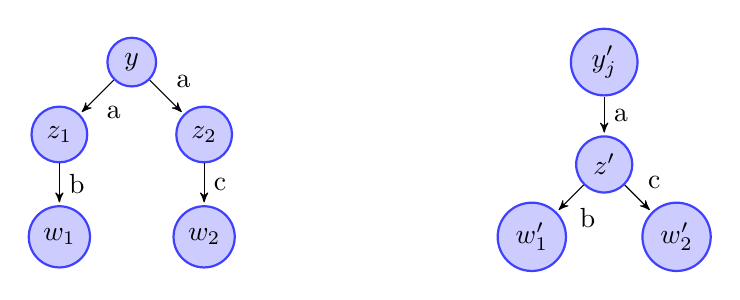
\begin{tikzpicture}[node distance=1.3cm,>=stealth',bend angle=45,auto]
  \tikzstyle{place}=[circle,thick,draw=blue!75,fill=blue!20,minimum size=6mm]
  \tikzstyle{red place}=[place,draw=red!75,fill=red!20]
  \tikzstyle{transition}=[rectangle,thick,draw=black!75,
  			  fill=black!20,minimum size=4mm]
  \tikzstyle{every label}=[red]

  \begin{scope}[xshift=0cm]
    \node [place] (t) {$y$};
    \node [place] (a) [below left of=t] {$z_1$}
      edge [pre]  node[swap] {a}                 (t);
    \node [place] (a2) [below right of=t] {$z_2$}
      edge [pre]  node[swap] {a}                 (t);
    \node [place] (b) [below of=a] {$w_1$}
      edge [pre]  node[swap] {b}                 (a);
    \node [place] (c) [below of=a2] {$w_2$}
      edge [pre]  node[swap] {c}                 (a2);
  \end{scope}  
  \begin{scope}[xshift=6cm]
    \node [place] (t) {$y'_j$};
    \node [place] (a) [below of=t] {$z'$}
      edge [pre]  node[swap] {a}                 (t);
    \node [place] (b) [below left of=a] {$w'_1$}
      edge [pre]  node[swap] {b}                 (a);
    \node [place] (c) [below right of=a] {$w'_2$}
      edge [pre]  node[swap] {c}                 (a);
  \end{scope}  
\end{tikzpicture}
\caption{Worked Example of $\mathsf{neg}$}
\end{figure}

Consider $y$ and $y'_j$ as in Fig.1.
One formula that is true in $y'_j$ but not in $y$ is
\[
\langle a \rangle (\langle b \rangle \top \land \langle c \rangle \top)
\]
Now:
\begin{eqnarray}
\mathsf{neg}(y, \langle a \rangle (\langle b \rangle \top \land \langle c \rangle \top)) & = & \nonumber \\
\bigwedge\limits_{y \xrightarrow{a} z} \langle a \rangle \mathsf{neg}(z, \langle b \rangle \top \land \langle c \rangle \top) & = & \nonumber \\
\langle a \rangle \mathsf{neg}(z_1, \langle b \rangle \top \land \langle c \rangle \top) \land \langle a \rangle\mathsf{neg}(z_2, \langle b \rangle \top \land \langle c \rangle \top) & = & \nonumber \\
\langle a \rangle (\langle b \rangle \top \land \mathsf{neg}(z_1, \langle c \rangle \top)) \land \langle a \rangle\mathsf{neg}(z_2, \langle b \rangle \top \land \langle c \rangle \top) & = & \nonumber \\
\langle a \rangle (\langle b \rangle \top \land \mathsf{neg}(z_1, \langle c \rangle \top)) \land \langle a \rangle(\mathsf{neg}(z_2, \langle b \rangle \top) \land \langle c \rangle \top) & = & \nonumber \\
\langle a \rangle (\langle b \rangle \top \land \fBang \{b\}) \land \langle a \rangle(\mathsf{neg}(z_2, \langle b \rangle \top) \land \langle c \rangle \top) & = & \nonumber \\
\langle a \rangle (\langle b \rangle \top \land \fBang \{b\}) \land \langle a \rangle(\fBang \{c\} \land \langle c \rangle \top) & & \nonumber
\end{eqnarray}
The resulting formula is true in $y$ but not in $y'_j$.


\subsection{Discussion}
Consider the fragment of HML without negation:
\[
\phi ::= \top \fOr \phi_1 \land \phi_2  \fOr \langle a \rangle \phi
\]
Without negation, $p \equiv p'$ does \emph{not} entail $p \sim p'$, as Fig. 3 shows.
\begin{figure}[h]
\centering
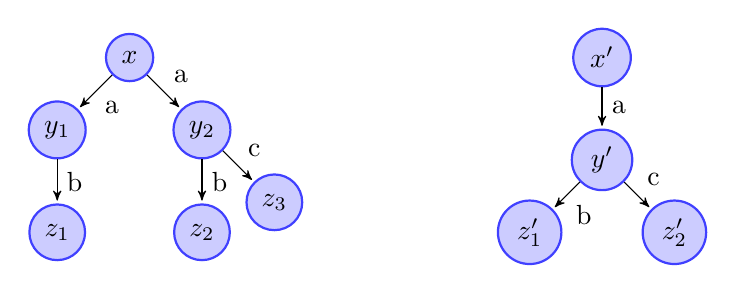
\begin{tikzpicture}[node distance=1.3cm,>=stealth',bend angle=45,auto]
  \tikzstyle{place}=[circle,thick,draw=blue!75,fill=blue!20,minimum size=6mm]
  \tikzstyle{red place}=[place,draw=red!75,fill=red!20]
  \tikzstyle{transition}=[rectangle,thick,draw=black!75,
  			  fill=black!20,minimum size=4mm]
  \tikzstyle{every label}=[red]

  \begin{scope}[xshift=0cm]
    \node [place] (w1) {$x$};
    \node [place] (e1) [below left of=w1] {$y_1$}
      edge [pre]  node[swap] {a}                 (w1);
    \node [place] (c) [below of=e1] {$z_1$}
      edge [pre]  node[swap] {b}                 (e1);
    \node [place] (e2) [below right of=w1] {$y_2$}
      edge [pre]  node[swap] {a}                 (w1);
    \node [place] (c) [below of=e2] {$z_2$}
      edge [pre]  node[swap] {b}                 (e2);
    \node [place] (c) [below right of=e2] {$z_3$}
      edge [pre]  node[swap] {c}                 (e2);
  \end{scope}  
  \begin{scope}[xshift=6cm]
    \node [place] (t) {$x'$};
    \node [place] (a) [below of=t] {$y'$}
      edge [pre]  node[swap] {a}                 (t);
    \node [place] (b) [below left of=a] {$z'_1$}
      edge [pre]  node[swap] {b}                 (a);
    \node [place] (c) [below right of=a] {$z'_2$}
      edge [pre]  node[swap] {c}                 (a);
  \end{scope}  
\end{tikzpicture}
\caption{Without negation, $p \equiv p'$ does not entail $p \sim p'$}
\end{figure}
Here, $x \equiv x'$ - they both satisfy the sub formulae of $\langle a \rangle (\langle b \rangle \top \land \langle c \rangle \top)$.
But there is no bisimulation between $x$ and $x'$ ($y_1$ cannot be matched with $y'$ because $y'$ has an additional outgoing $c$-transition). 

If we remove negation, HML  is insufficiently expressive to distinguish between these two non-bisimilar models.
When we restore negation, we can distinguish between these models via the formula:
\[
\langle a \rangle \neg \langle c \rangle \top
\]
Similarly, EL is able to distinguish between these models via the formula:
\[
\langle a \rangle ! \{b\}
\]
EL, also, has the expressive capacity to distinguish between non-bisimilar models. If the LTSs are finitely-branching, it can simulate negation (in innermost scope) via the width restriction operator !

\section{Translating EL into FOL}

We will translate EL into a restricted fragment of FOL.
There are three types of predicate:
\begin{itemize}
\item
A 0-place predicate $\top$, which is true in all models.
\item
A set of two-place predicates $Arr_s(x, y)$, one for each $s \in \mathcal{S}$, where $x$ and $y$ are of type $State$. $Arr_s(x, y)$ is true if $x \xrightarrow{s} y$.
\item
A set of one-place predicates $Restrict_A$, one for each finite subset $A \subseteq \mathcal{S}$. 
$Restrict_{A}(x)$ is true if $\lambda(x) = A$.
\end{itemize}
With $x_1, x_2$ being state variables, $s$ a symbol in $\mathcal{S}$, and $A$ ranging over subsets of $\mathcal{S}$, our restricted fragment of FOL has sentences of the form:
\[
\phi ::= \top \fOr Arr_{s}(x_1, x_2)\fOr Restrict_A(x_1) \fOr \phi_1 \land \phi_2 \fOr \exists x_1 . \phi 
\]
Notice that this fragment of FOL has no negation, disjunction, implication, or universal quantification.

The translation of an EL formula is relative to a variable $x$ (which will be instantiated to the particular state at which we are evaluating the formula):
\begin{eqnarray}
T_x(\top) & = & \top \nonumber \\
T_x(\phi_1 \land \phi_2) & = & T_x(\phi_1) \land T_x(\phi_2) \nonumber \\
T_x(\langle s \rangle \phi) & = & \exists y \; . \; Arr_s(x,y) \land T_y(\phi) \nonumber \\
T_x(\fBang A) & = & Restrict_A(x) \nonumber
\end{eqnarray}
So, for example:
\[
T_x(\langle a \rangle \top \land \fBang \{a\}) = \exists y \; . \; Arr_a(x,y) \land \top \land Restrict_{\{a\}}(x)
\]

\subsection{Discussion}
An EL formula is translated into a FOL formula of the complexity $\exists^*$, relative to a state $x$.
Checking that $\phi \models \psi$ requires calculating the validity of a FOL formula of the form:
\[
\forall (\exists^* \rightarrow \exists^*)
\]
Because our FOL formulae use no negation, disjunction, or implication, this can be done in linear time as follows:

First check if $T_x(\phi)$ is consistent.
This is done by conjoining $T_x(\phi)$ to a set of conditionals of the form:
\[
Restrict_A(x) \land Arr_a(x,y) \rightarrow \bot
\]
for each $a \in \mathsf{sym}(\phi)-A$ and each $A$ appearing in a formula $!A$ in $\phi$.
Here, $\mathsf{sym}(\phi)$ is the set of symbols in $\phi$.

$T_x(\phi)$ is inconsistent if 
\[
T_x(\phi) \land \bigwedge_{A \in \phi, a \in\mathsf{sym}(\phi)-A} Restrict_A(x) \land Arr_a(x,y) \rightarrow \bot \; \models \; \bot
\]
If $\phi$ is not consistent, then $\phi \models \psi$ is valid.
If $\phi$ is consistent, then construct the skolemized version of $T_x(\phi)$. 
Now $\phi \models \psi$ iff the skolemized version of  $T_x(\phi)$ is a witness for $T_x(\psi)$. 

\section{Comparing EL with Hennessy-Milner Logic}
\subsection{Syntax}
Given a set $\mathcal{S}$ of symbols, with $s$ ranging over $\mathcal{S}$, the sentences of Hennessy-Milner Logic (HML) are given by:
\[
\phi ::= \top \fOr \phi_1 \land \phi_2 \fOr \langle s \rangle \phi \fOr \neg \phi 
\]
\subsection{Semantics}
A {\bf Labelled Transition System} (LTS) is a pair $(\mathcal{W}, \rightarrow)$, where $\mathcal{W}$ is a set of states, and $\rightarrow$ is a set of transition relations: $\rightarrow \; \subseteq \; \mathcal{W} \times S \times \mathcal{W}$.
We write $x \xrightarrow{s} y$ to abbreviate $(x,s,y) \in \rightarrow$.

A {\bf pointed LTS} is a pair $(l, w)$, where $l$ is a LTS $(\mathcal{W}, \rightarrow)$ and $w$ is a distinguished state $w \in \mathcal{W}$.

A sentence of HML is evaluated in a pointed LTS $(l, w)$:
\begin{eqnarray}
(l,w) & \models & \top \nonumber \\
(l,w) & \models & \phi_1 \land \phi_2 \mbox{ iff } (l,w)  \models \phi_1 \mbox { and } (l,w) \models \phi_2 \nonumber \\
(l,w) & \models & \langle s \rangle \phi \mbox{ iff there is a } w \xrightarrow{s} w' \mbox { such that } (l,w') \models \phi \nonumber \\
(l,w) & \models & \neg \phi \mbox{ iff } (l,w)  \nvDash \phi \nonumber
\end{eqnarray}

\subsection{Translating EL into HML}
The only differences between EL and HML are:
\begin{itemize}
\item
Syntactically, EL has the transition-restriction operator ($!$) instead of logical negation ($\neg$)
\item
Semantically, an EL model has an additional node-labelling, describing the allowable transitions from each vertex
\end{itemize}
We can translate formulae of EL into HML using the function $t$:
\begin{eqnarray}
t(\top) & = & \top \nonumber \\
t(\phi_1 \land \phi_2) & = & t(\phi_1) \land t(\phi_2) \nonumber \\
t(\langle s \rangle \phi) & = & \langle s \rangle t(\phi) \nonumber \\
t(! A) & = & \bigwedge_{s \in S - A} \neg \langle s \rangle \top \nonumber
\end{eqnarray}
If $\mathcal{S}$ is an infinite set, then the translation of a $!$ formula will be an infinitary sentence.
If $\mathcal{S}$ is finite, then the size of the HML formula will be of the order of $n * |\mathcal{S}|$ larger than the original EL formula (where $n$ is the number of $!$ operators occurring in the EL formula).




\end{document}

